\chapter{機能}\label{cha:Function}

本章では、本研究で試作したモータ特性表自動生成ツールの機能について説明する。

モータ特性表自動生成ツールは、OpenModelicaで、Modelica言語にて作成したモータのモデルをシミュレーションした時に、
出力されるcsvファイルを読み込み、実行することによって、モータ特性表を生成する。\\

\section{対応するモデル}\label{taioumodel}
試作したモータ特性表自動生成ツールでは、以下のModelicaモデルのシミュレーション結果に対応する。
\begin{itemize}
	\item モータ単体のModelicaモデル
	\item モータ単体のModelicaモデルをサブシステムとするモデル
\end{itemize}
なお、今回はモータの中でもブラシ付きDCモータに対応する。\\
以降、上記のモデルについて具体的に説明する。

\subsection{モータ単体のModelicaモデル}\label{sec:sub1}
モータ単体のModelicaモデルとは、電源部品、抵抗部品、インダクター部品、起電力部品、慣性部品、接地部品を持つモデルのことである。\\
上記6つの部品が必要な理由は、ブラシ付きDCモータの等価回路\cite{等価回路}をModelica言語で表す際に、
使用する部品\cite{modelicaシステム本}だからである。\\
各部品で使用するMSLを表\ref{tab:MSL}に、ブラシ付きDCモータの等価回路図を図\ref{fig:touka}に、
モータ単体のModelicaモデルの例を図\ref{fig:tantai_model}に、
図\ref{fig:tantai_model}のModelicaコードを図\ref{fig:tantai_modelica}に示す。

\begin{table}[t]
	\centering
	\caption{MSL対応表}
	\begin{tabular}{|c|c|} \hline
	  部品名 & 使用するMSL \\ \hline \hline
	  電源部品 & Modelica.Electrical.Analog.Sources \\ \hline
	  抵抗部品 & Modelica.Electrical.Analog.Basic \\ \hline
	  インダクター部品 & Modelica.Electrical.Analog.Basic \\ \hline
	  起電力部品 & Modelica.Electrical.Analog.Basic \\ \hline
	  慣性部品 & Modelica.Mechanics.Rotational.Components \\ \hline
	  接地部品 & Modelica.Electrical.Analog.Basic \\ \hline
	\end{tabular}
	\label{tab:MSL}
  \end{table}
 
\begin{figure}[t]
	\centering
	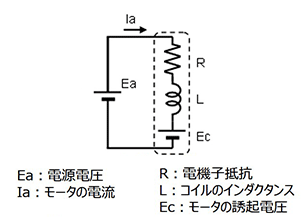
\includegraphics[width=7cm]{./Image/touka.png}
	\caption{ブラシ付きDCモータの等価回路}
	\label{fig:touka}
  \end{figure}

\begin{figure}[t]
  \centering
  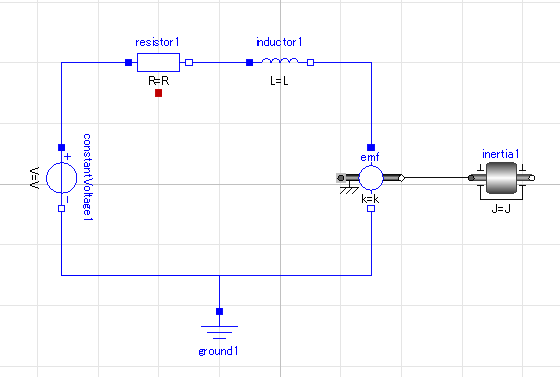
\includegraphics[width=8cm]{./Image/tantai_model.png}
  \caption{モータ単体のModelicaモデルの例}
  \label{fig:tantai_model}
\end{figure}

\begin{figure}[t]
	\centering
	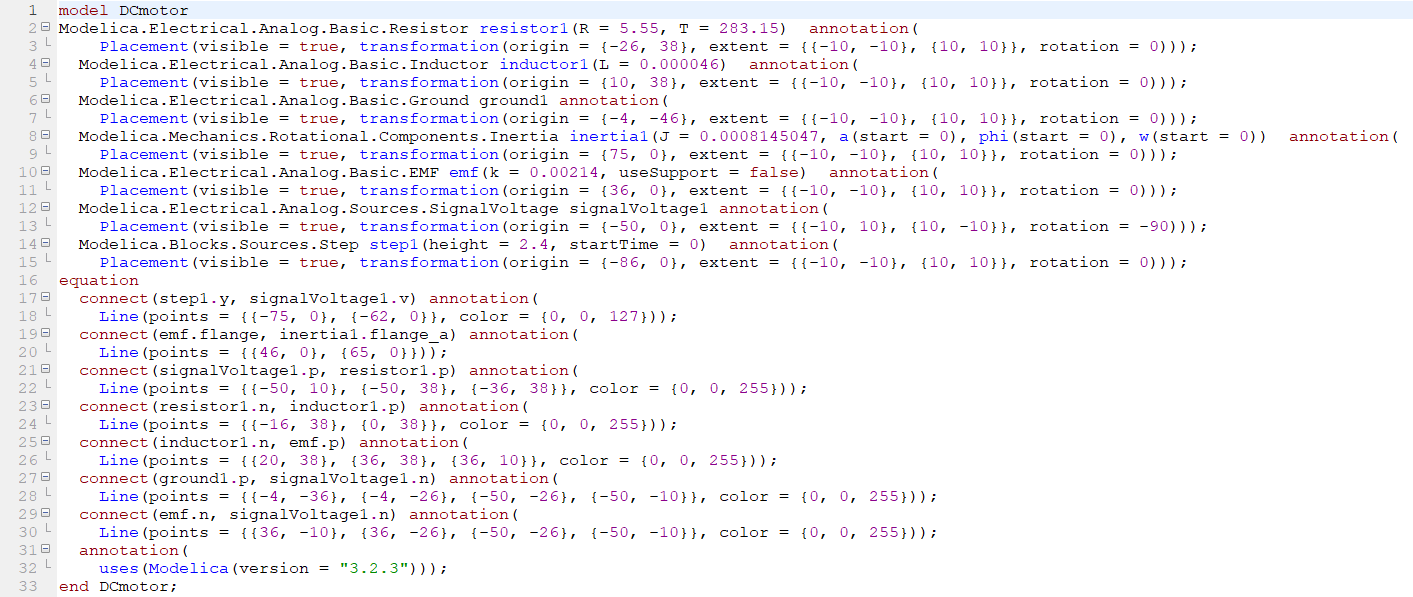
\includegraphics[width=16.5cm,height=8cm]{./Image/tantai_modelica.png}
	\caption{図\ref{fig:tantai_model}のModelicaコード}
	\label{fig:tantai_modelica}
  \end{figure}


\subsection{モータ単体のModelicaモデルをサブシステムとするモデル}\label{sec:sub2}
モータ単体のModelicaモデルをサブシステム\cite{modelicaシステム本}とするモデルとは、
\ref{sec:sub1}節で説明したモータ単体のModelicaモデルを一つのサブシステムとして書いたモデルのことである。\\
例として、DCモータのサブシステムを用いたDCモータサーボのモデルを図\ref{fig:submodel}に、図\ref{fig:submodel}の
Modelicaコードを図\ref{fig:sub_modelica}に示す。

\begin{figure}[t]
	\centering
	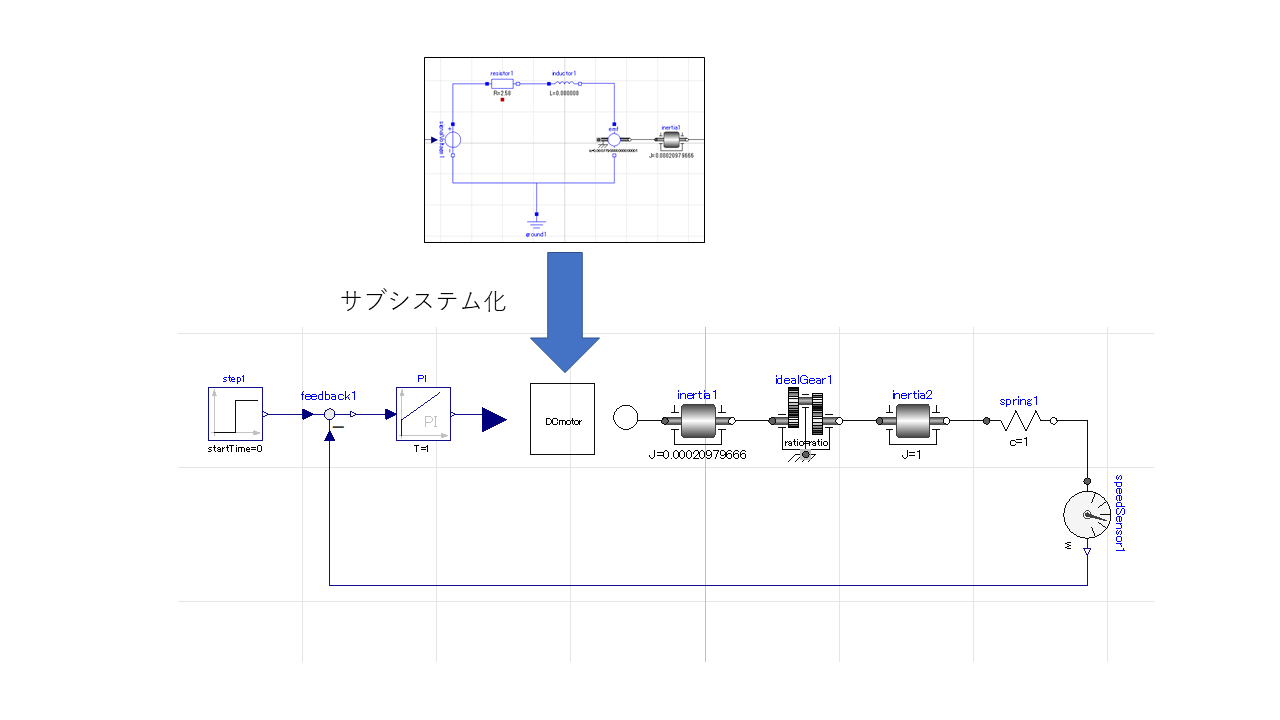
\includegraphics[width=16.5cm,height=10cm]{./Image/submodel_pack.png}
	\caption{DCモータサーボのモデル}
	\label{fig:submodel}
  \end{figure}

  \begin{figure}[t]
	\centering
	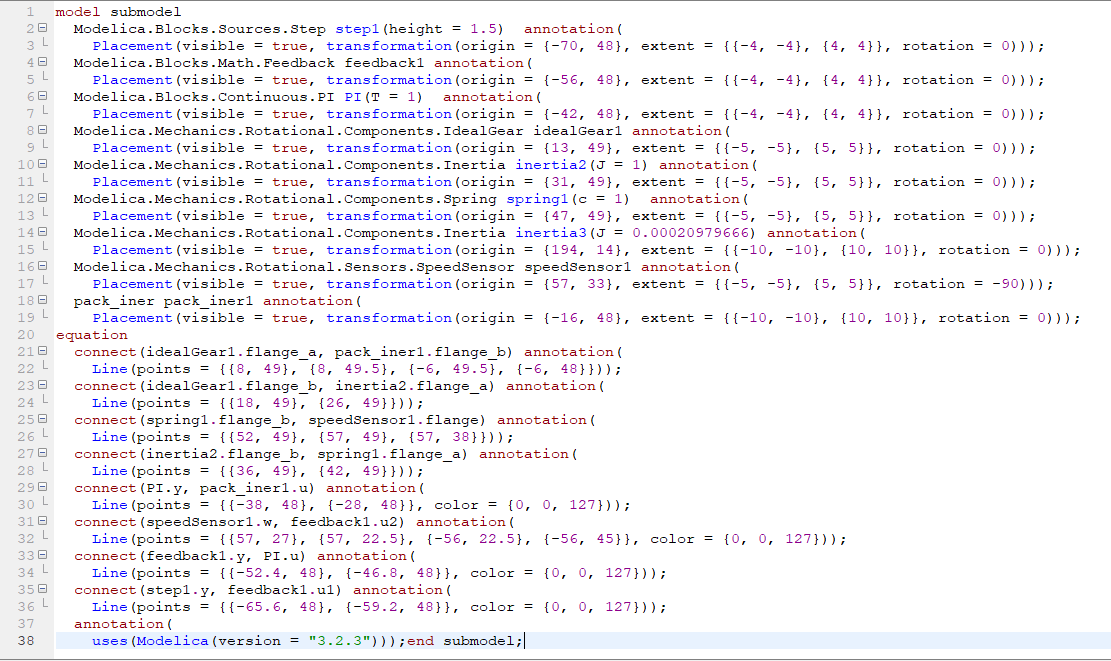
\includegraphics[width=16.5cm,height=10cm]{./Image/sub_modelica.png}
	\caption{図\ref{fig:submodel}のModelicaコード}
	\label{fig:sub_modelica}
  \end{figure}

  \clearpage

  \section{モータ特性表生成}\label{kenkyu_mokuteki}
今回試作したモータ特性表自動生成ツールは次の9個の要素を持つモータ特性表を生成する。

\begin{itemize}
	\item 始動電流 mA
	\item 停動トルク mNm
	\item 最大効率 \%
	\item 定格トルク mNm 
	\item 定格回転数 rpm
	\item 定格電流 mA
	\item 定格出力 W
	\item 定格電圧 V
	\item 最大回転数 rpm 
\end{itemize}

図\ref{fig:tantai_model}のモデルをシミュレーションした時に、OpenModelicaから出力されるcsvファイルの一部を
図\ref{fig:simyu_csv}に、図\ref{fig:simyu_csv}から作成できる特性表を図\ref{fig:tokuseihyou}に示す。

  \begin{figure}[t]
	\centering
	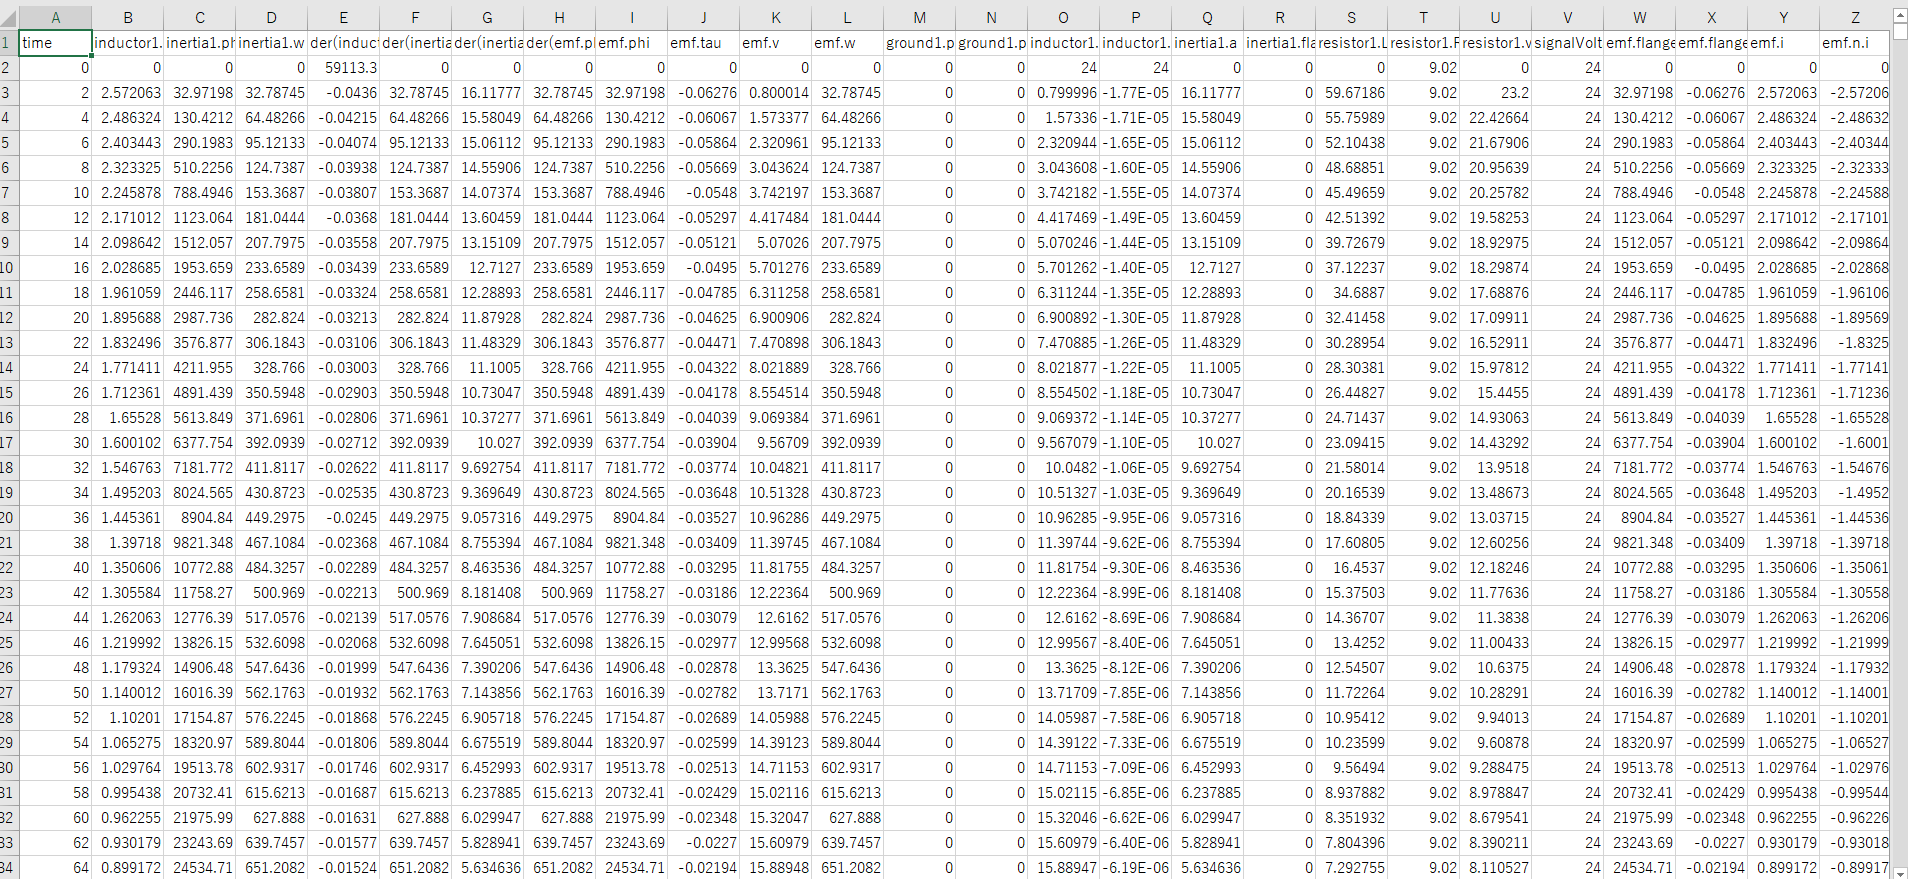
\includegraphics[width=16.5cm,height=9cm]{./Image/simyu_csv.png}
	\caption{図\ref{fig:tantai_model}のシミュレーション結果のcsvファイルの一部}
	\label{fig:simyu_csv}
  \end{figure}

  \begin{figure}[t]
	\centering
	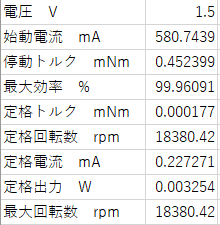
\includegraphics[width=5cm]{./Image/chara_table.png}
	\caption{図\ref{fig:simyu_csv}のcsvファイルから作成した特性表}
	\label{fig:tokuseihyou}
  \end{figure}